\section{N2Sky Components}\label{N2Sky Components}

In the concept of N2Sky lies minimalistic and modern design. Dimmed tones of the UI components are used to make end-user to feel like he is using professional expert system. Every component and element was carefully thought out in order to keep the same atmosphere throw the whole application. 

\subsection{User Interface Components}\label{User Interface Components}

Familiar elements and components helps users easier navigate through the application. It is important to have common components and elements and do not mixup all together. Every component and every GUI element should have self-describing purpose. Building user interface components and elements is pretty same as develop some UML digram. It is possible to group common parts and maximise reusability \cite{mod_ui_book}. 

It is important to consider the multiple end-users, devices, platforms as well as environments will be used. Throw heterogeneous context only needed elements has to be displayed. It is necessary to make view prototypes to determine if the particular component comfortable and easy to use \cite{Martinez2017}. 

\subsubsection{User Interface Elements}\label{User Interface Elements}

It is possible to divide all UI elements into groups \cite{intelligent_support}:

\begin{description}
\item[Input Controls.] Input controls determine user input action. Input actions are keyboard typing or mouse clicking.  Following UI elements are the part of input controls: 
\begin{itemize}
\item Checkboxes
\item Radio buttons 
\item Dropdown Lists
\item List boxes
\item Buttons
\item Toggles
\item Text fields
\item Date field
\end{itemize}
\item[Navigational Components.] Navigation between page views. Navigational components includes also some particular request from and to user. Following UI elements are the parts of navigational components:
\begin{itemize}
\item Breadcrumb 
\item Slider
\item Search field
\item Pagination
\item Slider
\item Tags
\item Icons
\end{itemize}
\item[Informational Components.] This components are addition to workflows. It can help user to perform some actions or they can to inform user, that the action will occur or already occurred. Informational Components contains of following UI elements:
\begin{itemize}
\item Tooltips
\item Icons
\item Progress bar
\item Notifications
\item Message boxes
\item Modal windows
\end{itemize}
\item[Containers.] Containers are components, which are hiding additional information or not focused information, where user need to perform action in order to see it.   
\begin{itemize}
\item Accordion
\item Semihidden elements
\end{itemize}
\end{description}

\subsubsection{UI Elements in N2Sky}\label{UI Elements in N2Sky}

N2Sky supports almost all common web user interface elements. Every element was developed in order do be reusable. Since N2Sky supports responsive design, the UI elements should also be responsive. Every UI element is absolute customised. Following UI elements were created:

\begin{description}
\item[Accordion]  Accordion is a list of items, which is accessible on mouse click. In N2Sky accordion works more like a modal window. With this kind of functionality other data, which surround accordion will not be stretched or squeezed, but will appear on top of elements ``Fig.~\ref{fig:accordion}''.: 

\begin{figure}[htbp]
\begin{center}
  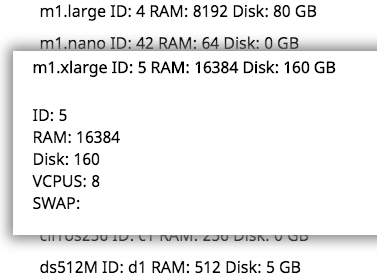
\includegraphics[scale=0.75]{components/3/components/accordion.png}
  \caption{Customised N2Sky accordion UI element}
  \label{fig:accordion}
\end{center}
\end{figure}

\item[Buttons.] Idea behind was to make buttons more interactive and understandable to use ``Fig.~\ref{fig:button_inactive}''. Buttons contain caption and icon in SVG format in order to support high quality image in all devices.

Buttons are using on hover animation. When mouse over the button, then button icon slide to the middle to show that action can be performed ``Fig.~\ref{fig:button_active}''. 

\begin{figure}[htbp]
\begin{center}
  
\includegraphics[scale=0.55]{components/3/components/button_inactive.png}
  \caption{Customised N2Sky button UI element}
  \label{fig:button_inactive}
\end{center}
\end{figure}


\begin{figure}[htbp]
\begin{center}
  
\includegraphics[scale=0.55]{components/3/components/button_active.png}
  \caption{Customised N2Sky button UI element animation}
  \label{fig:button_active}
\end{center}
\end{figure}

\item[Icons.] In N2Sky all icons are in Scalable Vector Graphics (SVG) format. With SVG the icons does not loosing quality in any device \cite{Cagle2005}. Since it is a vector graphic it easy to edit an icon with programming language code. N2Sky Logo, which is represented in ``Fig.~\ref{fig:logo}'',  is also made in SVG format. 

\begin{figure}[htbp]
\begin{center}
  
\includegraphics[scale=0.55]{components/3/components/logo.png}
  \caption{Customised N2Sky logo in SVG format}
  \label{fig:logo}
\end{center}
\end{figure}

Is it possible to import code in some graphical vector editor in order change colour, path (vector graphic itself), metadata etc. Following code demonstrate N2Sky Logo in SVG format. The whole vector path was shortened.

\begin{lstlisting}
<?xml version="1.0" standalone="no"?>
<!DOCTYPE svg PUBLIC "-//W3C//DTD SVG 20010904//EN"
        "http://www.w3.org/TR/2001/REC-SVG-20010904/DTD/svg10.dtd">
<svg version="1.0" xmlns="http://www.w3.org/2000/svg"
     width="266.000000pt" height="267pt" viewBox="0 0 266 267"
     preserveAspectRatio="xMidYMid meet">
    <metadata>
        N2Sky Logo. 2018
    </metadata>
    <g transform="translate(0.000000,267.000000) scale(0.100000,-0.100000)"
       fill="#6b6b6b" stroke="none">
        <path d="M1302 2638 c-9 -9 -12 -83 -12 -270 0 -245 -1 -259
-37 -26 -170 21 -63 23 -132 46 -152 52 -23 7 -38 17 -38 27 1
80 222 90 255 87 284 -2 23 -9 32 -25 34 -27 4 -46 -23 -72 -106 
-77 -34 -95 -8 -18 -22 -51 -32 -74 -10 -24 -21 -43 -25 -43 -5 0 -30 
76 -76 118 -100 136 -128 92 -12 -20 -10 -26 101 -219 35 -60 109 

...

-18 74 -40 36 -22 67 -40 70 -40 11 0 253 -152 269 -169 11 -12 15 -27 12 
-36 26 -103 -14 -32 -19 -60 -35 -62 -35 -3 0 -34 -18 -70 -40 -36 -22 -68
-40 -70 -40 -3 0 -22 -11 -43 -23 -142 -90 -172 -96 -201 -39 -20 40 -47 168
-55 268 l-5 61 122 22 c67 13 156 30 197 38 85 16 106 30 95 63 -7 21 -11 22
-69 16 -33 -4 -88 -10 -121 -15 -178 -26 -178 -26 -170 -1 4 13 21 46 37 74
57 100 63 116 52 134 -6 9 -22 17 -34 17 -24 0 -47 -33 -130 -180 -75 -132
-74 -130 -61 -206 6 -38 16 -102 21 -141 6 -40 15 -98 20 -129 6 -30 10 -72
10 -93 l0 -38 -162 4 c-151 3 -167 5 -212 28 -82 43 -86 57 -86 320 l0 226 38
34 c21 19 53 47 72 61 19 14 49 39 67 55 17 16 54 47 82 69 60 49 79 79 65
103 -18 28 -47 25 -84 -10 -20 -18 -52 -45 -72 -60 -20 -15 -42 -34 -50 -41
-23 -23 -92 -67 -105 -67 -10 0 -13 27 -13 104 0 57 -3 111 -6 120 -7 19 -45
21 -62 4z"/>
    </g>
</svg>
\end{lstlisting}

\item[Notification messages.] Notification messages are the part of information component. In N2Sky used two types of notification messages: 
\begin{itemize}
\item Waring message, which tells, that something goes wrong as it shown in ``Fig.~\ref{fig:notif_warning}''. It can be error in the application as well as user workflow error. 
\item Informational message that gives information about event which will occur or already occurred as it shown in ``Fig.~\ref{fig:notif_info}''.
\end{itemize}


\begin{figure}[htbp]
\begin{center}
  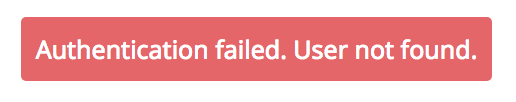
\includegraphics[scale=0.65]{components/3/components/notif_warning.png}
  \caption{Customised N2Sky warning message UI element}
  \label{fig:notif_warning}
\end{center}
\end{figure}

\begin{figure}[htbp]
\begin{center}
  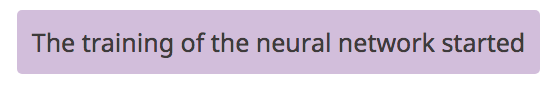
\includegraphics[scale=0.65]{components/3/components/notif_info.png}
  \caption{Customised N2Sky informational message UI element}
  \label{fig:notif_info}
\end{center}
\end{figure}

\item[Navigation.] In N2Sky user can navigate to another one page or change part of the page view via tabs, navigation buttons and menus. 
Navigation elements are bind into group of element or UI components. Following navigation component which is shown in ``Fig.~\ref{fig:nav}'', contains navigation elements as well functional icon. 
\end{description}

\begin{figure}[htbp]
\begin{center}
  
\includegraphics[scale=0.65]{components/3/components/nav.png}
  \caption{Customised N2Sky navigation UI element}
  \label{fig:nav}
\end{center}
\end{figure}

Navigation bars can contain tabs, buttons, icons and non-functional text. ``Fig.~\ref{fig:nav_bar}'' shows navigation bar an custom table. 

\begin{figure}[htbp]
\begin{center}
  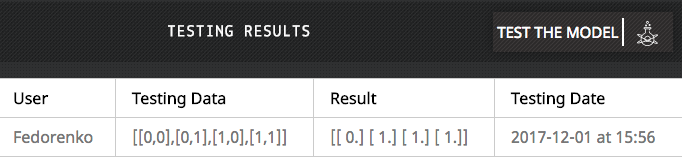
\includegraphics[scale=0.65]{components/3/components/nav_bar.png}
  \caption{Customised N2Sky navigation bar with a table}
  \label{fig:nav_bar}
\end{center}
\end{figure}

\subsubsection{UI Components in N2Sky}\label{UI Components in N2Sky}

Groups of UI elements form UI components. Components, like elements, are also fully reusable, only context of components is changing. Following custom UI components were developed in N2Sky: 

\begin{description}
\item[Grid Item Component.] Grid in N2Sky is responsive. It can change positions and size of grid items like it shown in ``Fig.~\ref{fig:grid_item}''. 

\begin{figure}[htbp]
\begin{center}
  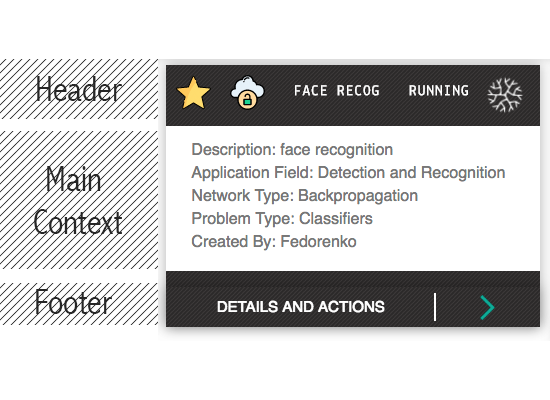
\includegraphics[scale=0.65]{components/3/components/grid_item.png}
  \caption{Responsive N2Sky Grid Item UI comonent}
  \label{fig:grid_item}
\end{center}
\end{figure}


Grid item contains following UI element: 
\begin{description}
\item[Header. ] Header is the first component on which the user focuses, that is why it should be short, but highlighted. Following UI elements are included: 
\begin{itemize}
\item Functional icons-buttons on the left side (optional)
\item Title of grid item (mandatory)
\item  Non-functional icons (optional)
\end{itemize}
\item[Main context. ] Component, which contains context information. This component can be fully customised. It is possible to put there list of items, plain text or even image.
 \item[Footer. ] Footer is an optional element and contains only button UI element. 
\end{description}

\item[Main navigation menu.] Every N2Sky view use main navigation menu, namely menu is injected in abstract view, which is extended by all other view components. Menu has a menu items, which contain caption and an icon. As it was mentioned before, N2Sky has two modules: administration module and main application module. Both modules are represented in menu and menu items visibility depending on logged-in user permission. 
Menu for arbitrary user is shown in ``Fig.~\ref{fig:menu_user}''  and has following menu items:

\begin{itemize}
\item Profile 
\item N2Sky Dashboard
\item Available neural networks
\item Models repository
\end{itemize}

 
 \begin{figure}[htbp]
\begin{center}
  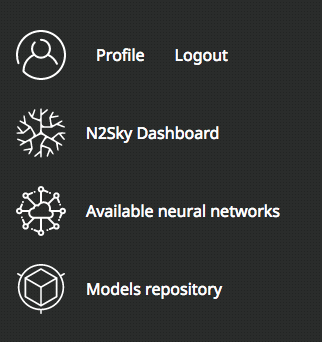
\includegraphics[scale=0.65]{components/3/components/menu_user.png}
  \caption{N2Sky Main Navigation Menu for arbitrary user}
  \label{fig:menu_user}
\end{center}
\end{figure}

If end-user is a system administrator, he can see additional menu form administration module as is demonstrated in ``Fig.~\ref{fig:menu_admin}'. This menu contains dropdown submenus: 

\begin{itemize}
\item OpenStack Dashboard
\item Cloudify Dashboard
\item Alert System
\item Dashboards Settings
\end{itemize}


 \begin{figure}[htbp]
\begin{center}
  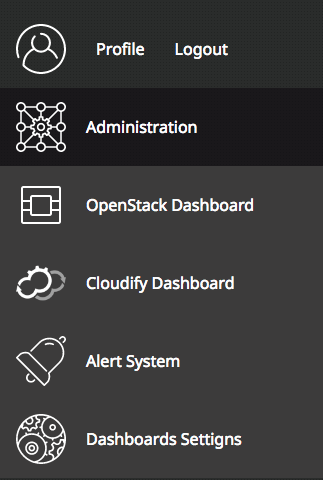
\includegraphics[scale=0.65]{components/3/components/menu_admin.png}
  \caption{N2Sky Main Navigation Menu for system administrator}
  \label{fig:menu_admin}
\end{center}
\end{figure}

\item[Modal windows.] N2Sky use modal windows almost in every view as it shown in ``Fig.~\ref{fig:modal}'. Modals are responsive and touch screen friendly. It has 3 elements:
\begin{itemize}
\item Title (mandatory)
\item Context (mandatory)
\item Submit button (optional)
\end{itemize}

 \begin{figure}[htbp]
\begin{center}
  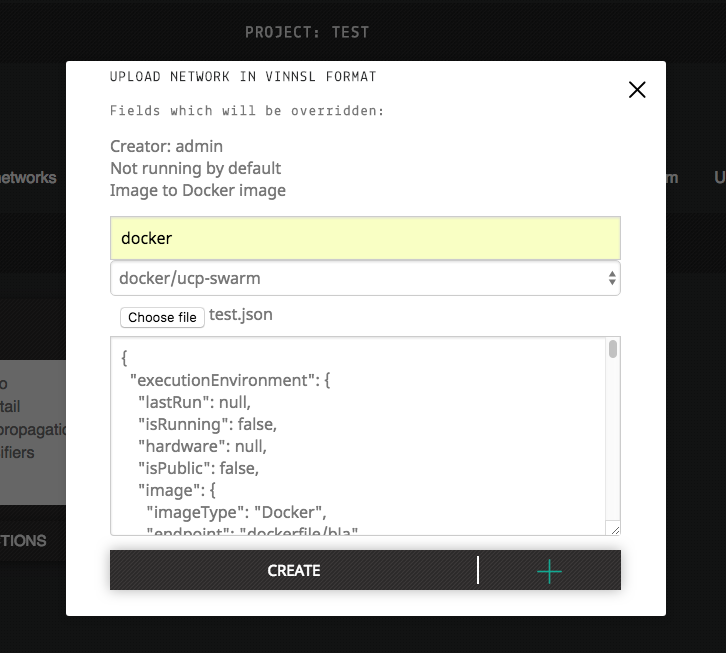
\includegraphics[scale=0.65]{components/3/components/modal.png}
  \caption{N2Sky Modal Window UI component}
  \label{fig:modal}
\end{center}
\end{figure}

Modals can be used to represent form as well for informational purposes. When modal is open the background is dunned in order to focus user on modal context. Modal context itself can be fully custom. It is possible to put any UI element in context.



\end{description}



\subsection{N2Sky Services}\label{N2Sky Services}

\subsection{Continuous Monitoring System}\label{Continuous Monitoring System}
\hl{TODO}
\subsubsection{Monitoring requirements}\label{Monitoring requirements}

The base monitoring system is readable and understandable representation of the graph. Graphs allow you to see objects beaning monitored and recognise metric from these objects. 
The good monitoring graph gives meaningful description, helps quickly to detect and determine issues via representation. This kind of graph should serve as a motivation for action to solve problems. 
There are some simple rules, which makes graphing well:

\begin{description}
\item[Consistency.] Representation should correctly reflect reality. All objects, which are represented on the graph, must be correlated with a real data on the machine. 
\item[Graphs need to make sense.]  All lines represented on the chart have to be readable and understandable.  Fake or unreadable information could cause problems. Metrics set should be small, one metric represent one object. There is no need to put multiple objects which are does not bind directly to one chart.
\item[Stacked area vs. multiline area.] Not every chart should have the same visual representation of the lines. Depending on the case we can decide which type of area to use.  If there are small time series with a high frequency it is better to use multiline area and stacked area on longer time series but with a bigger metric set respectively. 
\item[Understanding graph before starting to analyse it. ] Since there are going to be multiple charts with a different metrics we need to make sure that every user can understand the meaning of particular graph. Good naming, fulfilled contend and correct positioning are very important.
\item[Data hierarchy. ] It is important to define groups, metrics, data points and nested levels on the chart.  Groups help to bind similar objects together. Data points give information of time stamps. Metrics is actual graph representation. Nested level is multiple line metrics. All mentioned data should be visible and accessible. 
\item[Clarity.] Designing a chart it is important to take into consideration that there are multiple devices with a different screen resolution. Too many lines on limited space will make chart unreadable.  If there are lots of charts on one page it makes people confused what a meaning of this page. That is why it is a good practice to create multiple pages with grouped charts. 
\item[Perspective.] It is important to put graphs in such perspective so that any deviation will be easily noticeable. 
\item[Appeal.] All charts are people oriented, people today like simple and clean appearance of the applications and if an application has lots of charts they need to be with an appropriate design.  
\item[Control and managing.] It should be possible for any user to manipulate a graph. Either to change time series or remove some metric, customization of the graph makes the whole application more attractive.
\end{description}

\subsubsection{Applying Monitoring}\label{Applying Monitoring}
To build continues monitoring system there is need to user a toolkit with an active ecosystem.  Searching for a proper toolkit the toolkit should fulfilled some specific requirements that going to be use in N2Sky:
\begin{itemize}
\item Proper and self-describable metric name with a key pairs
\item Possibility to query metrics and join them in one graph.
\item Not resource-intensive
\item Support HTTP/HTTPS protocol
\item Collect and push to repository time series
\item Scalable
\end{itemize}

After researching it was decided to go for Prometheus Monitoring Toolkit. \hl{[1]} This tool support all requested requirements. One of most interesting feature is that Prometheus can be used on any UNIX environment. Since in Openstack multiple instance with a different operational system can be created, Prometheus will match exact our needs. 
Originally Prometheus was created by SoundCloud team in 2012. \hl{[2]} The core of monitoring application is Prometheus server, which collects time series data from the moment it was executed on environment as it shown in ``Fig.~\ref{fig:prometherus_arch}''. All components are written on Go \hl{[3]} language and support multiple modules for monitoring different environment metrics. 
To understand the nature of Prometheus it is necessary to explain its architecture. 

\begin{figure}[htbp]
\begin{center}
  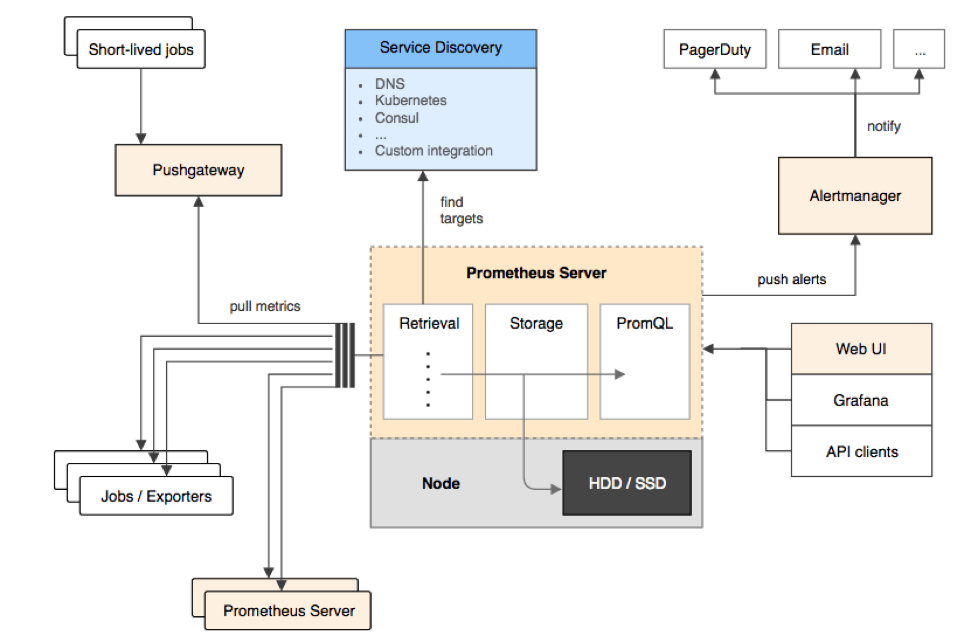
\includegraphics[width=\linewidth]{components/3/prometherus_arch.png}
  \caption{Prometheus monitoring architecture}
  \label{fig:prometherus_arch}
\end{center}
\end{figure}

The core Prometheus server pull all metrics from jobs which are instrumented, if the service is unavailable for instrumentation it can be pulled from push gateway. All metrics and logs data is stored locally so there is no distributed storage. It is possible to query this data to retrieve more specific information about particular metrics of joint metrics. N2Sky uses Prometheus API to build own customised dashboards. 
The common components of Prometheus architecture:
\begin{description}
\item[The Prometheus server.] This is the base element in the whole architecture. The server include services which collection, storing and retrieving nodes. The principle is scrapping or pulling. It means that the data fetched with some interval, which can me configured and stored accordantly as a time series. Prometheus support different modules, each module represents some node. The nodes expose these ports that Prometheus uses for retrieving the data. For example in N2Sky we are using Node Exporter Module which gives possibility to collect almost all essential data like CPU, RAM, HDD/SSD etc.
\item[Push gateway.] There are some nodes, which are not exposing these endpoints. In this case collection of the data throw Push gateway is possible.  Prometheus short-lived jobs are executed to capture the data and convert it to the time series that can be used by Prometheus.
\item [Alert Manager.]  Monitoring consist of multiple metrics, each metric can be analysed. It is possible to subscribe to particular metric in order to detect metric behaviour namely metric deviations. Alert Management System used for firing events, it is possible to receive alert notification over multiple channels like Emails, SMS, Push notification etc.
\end{description}

Metric notation 
Following example represent metric notation:
\begin{lstlisting}
node_filesystem_avail {method="GET", endpoint="/api/posts", status="200"}
\end{lstlisting}

The metric naming is always self-described.  Requested metric "node\_filesystem\_avail" means available free space in the filesystem.  Every operational system has different metic naming. N2Sky will propose list of available metrics. In curly brackets defined the type of request, an endpoint and expected HTTP response status.

After executing this query the data will be retrieved from logs and represent as a time series as it shown on ``Fig.~\ref{fig:monitoring_req}''.



\begin{figure}[htbp]
\begin{center}
  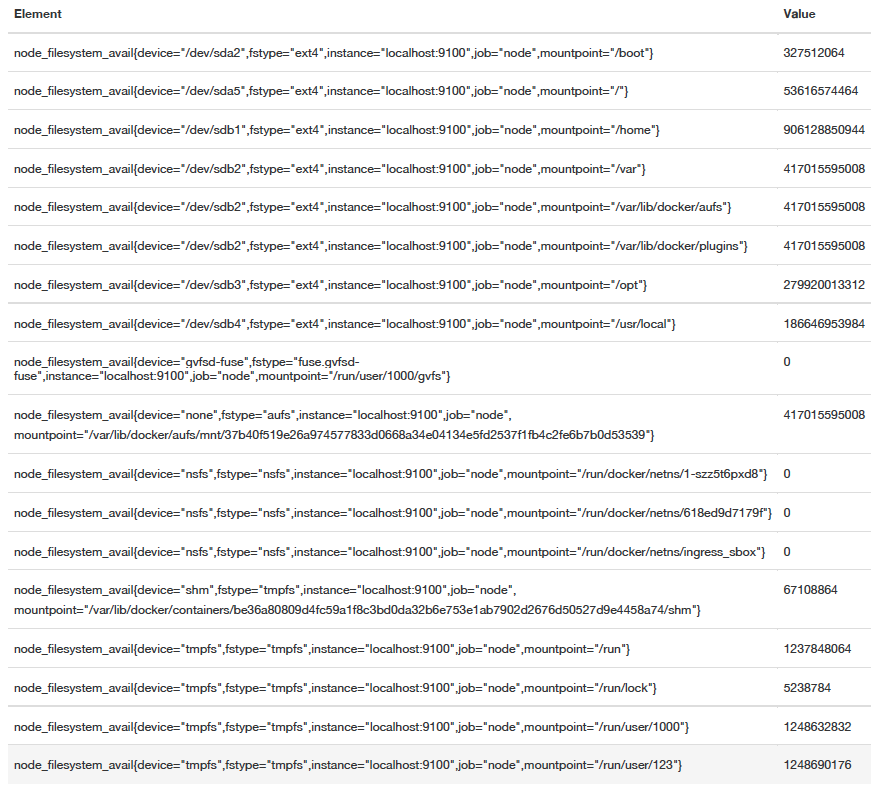
\includegraphics[width=\linewidth]{components/3/monitoring_req.png}
  \caption{Metric response}
  \label{fig:monitoring_req}
\end{center}
\end{figure}

One of the requirements to our monitoring system is scalability. One of the greatest features of Prometheus is that event if environment going to be overloaded it will generate the same amount of metrics anyway. Hence the amount of events is independent on amount on generated time series. 
Talking about requirements it is important to mention here that there is possibility to build joint metrics namely build multiple time series using this kind of metric:

\begin{description}
\item[Counter] The counter is a metric is representing a simple numerical value which can be incremented but not inverse. One of the typical examples is a number of expectations to be occurred. 
\item[Gauge] The gauge is a metric, which also represents a simple numerical value like counter, but it is bidirectional. It means that this value can be decremented. The common example is CPU usage, which can go up and down.
\item[Histogram] The histogram is a metric, which represent observations.  It is stored as a bucket, which can be pulled. Any bucket can be configured depending on the need. It can be sum of values or count of events, which are observed.
\item[Summary] The summary is a metric, which is similar to histogram but it calculates configurable quantities. 
\end{description}

\subsubsection{Integration with N2Sky}\label{Integration with N2Sky}

Prometheus supports query language, which is a key feature for this tool. The Prometheus query language, or promql, is an expressive. 
With Prometheus the self-described metric name can be choose. Prometheus converts all metric so that every human can understand what exactly particular metric means. Lets take a previous example with a metric "node\_filesystem\_avail". This metric will show the folders on root and available memory on each of it.

\begin{lstlisting}
	node_filesystem_avail 
		{device="/dev/sdb4",fstype="ext4",
		instance="localhost:9100",job="node",
		ssmountpoint="/usr/local"}
\end{lstlisting}

Following request means that on "/usr/local" 186.6 GB is available. 

There is also possibility to check a response code, which especially useful for alerting. 

\begin{lstlisting}
		node_filesystem_avail {status="500"}
\end{lstlisting}

This request returns some response code 500 namely internal server error. 

For building proper dashboard for monitoring it is important to provide customisation that is why Prometheus supports time duration:

\begin{itemize}
\item s - seconds
\item m - minutes
\item h - hours
\item d - days
\item w - weeks
\item y - years
\end{itemize}

Using the time duration with an offset it is possible to get exact metric on demand. 
Building query with a Prometheus can bring lots of advantages. For example there is query which use counter with a available node file system metric:

\begin{lstlisting}
topk( 3, sum(
		 rate(api_http_requests_total{status=500}[1h]
	) )
 by (endpoint)
 )
\end{lstlisting}

This query is already complicated, but it can be extended by multiple new rules and constrains. 

In N2Sky was developed monitoring service, which use microservices approach like in entire application. It was decided to get rid of complex queries and provide some intuitive way of creating metrics. 
First of all the time range add a complexity. It was decided that the user should give only time interval and step. Lets say the user want to see CPU load for a last hour with a step 30 seconds. It makes creation of metric more intuitive, no more range like "from", "to" and type of ranges. All this can be solved with a one simple request. 
Second part is a storing of metric. Instead of every time build a query the monitoring service saving requested by user metric. In this case every user will get his own customised metric. 
The service uses Mongo DB for storing the metric configuration. Every collection has it own schema. When a user make a request to save a metric the schema have to be filled with a requested by user data.

\subsubsection{Monitoring dashlet Design}\label{Monitoring dashlet Design}

Since there are multiple machine and services to monitor there was need to create a dedicated dashboard design.  At first lets take a look on the environments we have to monitor: 
\begin{description}
\item[Openstack Machine.]  It is dedicated machine, our cloud base for development and running instances.
\item[Openstack Instances.]   Virtual machines with a different OS.
\item[Docker Containers.]  Virtual machines in the Openstack instances.
\end{description}

One of the most important part in application design is to maximise reusability of the components. 


\subsection{Alerting Management System}\label{Alerting Management System}

Today the most trending subject in monitoring area is a prediction and automated detection. It makes people free from 24/7 managing, maintaining and monitoring system.
For monitoring we are using Prometheus tool. Since this tool saving constantly log data about system it is possible to reuse this logs to build an alert system. 
Prometheus tool provides an Alert Manager module. Natively this tool supports different notification methods like email notification or some request on Slack. 

\subsubsection{Alerting System Architecture}\label{Alerting System Architecture}

Since the Alert Manager is a part of Prometheus Tool it has its own binary. The idea behind is to have only one Alert Manager and have monitoring tool on multiple machines. If machine goes down or even Prometheus itself, the Alert Manager can catch and deliver this event. 
To understand how Alert Manager works it is essential to understand the architecture of the whole system ``Fig.~\ref{fig:alert_arch}''.

\begin{figure}[htbp]
\begin{center}
  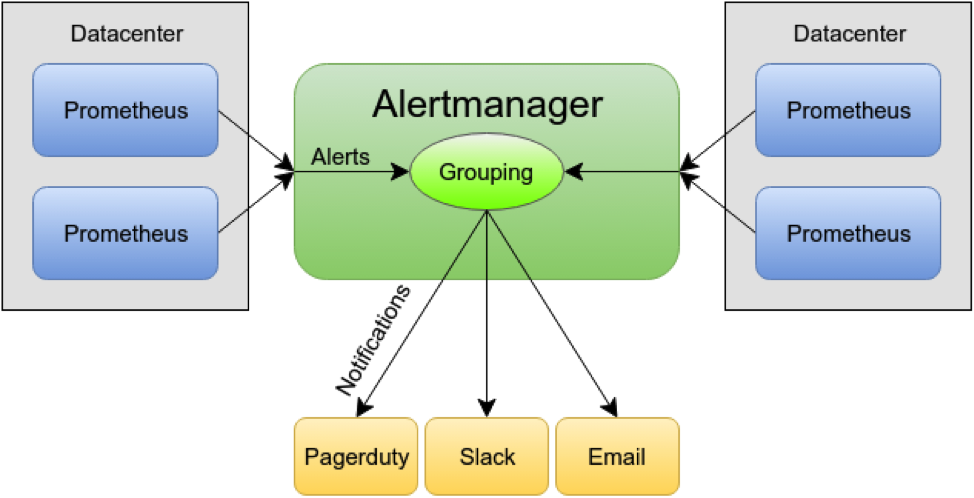
\includegraphics[width=\linewidth]{components/3/alert_arch.png}
  \caption{Alerting System Architecture}
  \label{fig:alert_arch}
\end{center}
\end{figure}

This architecture is a typical messaging platform. 
Messaging Service send messages between multiple clients. It is implement Producer-Consumer Pattern. In the Alert Manager Architecture the role of producer is taken by Prometheus Datacenter. Alert Manager consumes the messages. Consumer knows nothing about producer and just subscribe on event. With this approach it is possible to attach multiple producers. \hl{[Strategies for Integrating Messaging and Distributed Object Transactions https://link.springer.com/chapter/10.1007/3-540-45559-0\_16]}

Alerts can be collected in groups by datacenter. It means if an event occurs on multiple machines it can be packed into one notification and fired accordingly. 
In Prometheus configuration need to be setup only two things: reference on Alert Manager and Alert Rules. When Alert Manager consume an event it just dispatch it via notification ``Fig.~\ref{fig:alert_arch_detailed}''.. 

\begin{figure}[htbp]
\begin{center}
  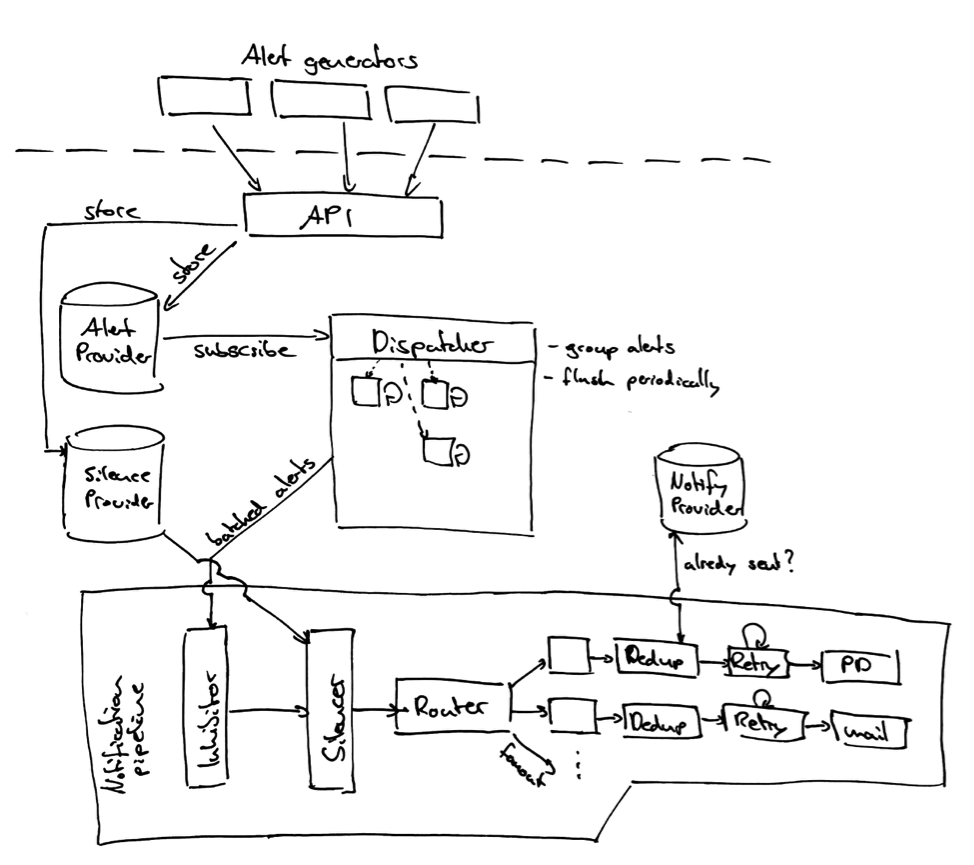
\includegraphics[width=\linewidth]{components/3/alert_arch_detailed.png}
  \caption{Communication within Alerting Management System}
  \label{fig:alert_arch_detailed}
\end{center}
\end{figure}

\subsubsection{Alert Rules}\label{Alert Rules}

As it was mention one of the main changes in Prometheus setup is to configure the alert rules. Every Prometheus Monitoring Tool can have it own alerting rules, which can be defined. There is also a possibility to reference on some common alerting rule for every monitoring system on every machine. 
Alerting rules are instructions to the monitoring system it can be user as well for alerting as for recording. 
Recording rules allows to pre-compute frequently needed expressions or expressions, which are resource or time consuming.  These rules are saving result in a new set of time series. It is like indexing this data, so that prevent expansive I/O methods. 
The rules are being executed sequentially with a predefined interval. 
With a alerting rules it is possible to define alert namely deviation by particular expression from Prometheus Tool and its exports (modules). It allows building an alert even on combined query. 
In case if Alert Manager is not available all alerts are saving into buffer. As soon Alert Manager online all events will be fired sequentially. 

\subsubsection{Integration with N2Sky}\label{Integration with N2Sky Alerting}

Alerting System is represented as a module in N2Sky. 
Alerting Client is the additional configuration upon Prometheus Monitoring System. When Prometheus will be executed it should have reference on Alerting System and its rules. 
Since the client should be installed on each OpenStack instance it was integrated into image snapshot. When the new instance will be spawned with a OpenStack snapshot, the client will be automatically executed there.  
Alerting Client fire alerts depending on configured rules. The rules can be created via user interface. Every alert has its severity level. Depending on it the fired events will be represented differently: 
?	Saverity 

\hl{TODO}

\subsubsection{Alerting System Design}\label{Alerting System Design}
\hl{TODO}



